% Документ принадлежит классу article
%\documentclass[a5paper,8pt]{article} 

% Документ принадлежит классу article, боковые отступы для двустраничной печати.
 \documentclass[twoside,a5paper,8pt]{article}

% нормальный юникод и русский язык
\usepackage{cmap}
\usepackage[T2A]{fontenc}
\usepackage[utf8]{inputenc} 
\usepackage[russian,english]{babel} % Пакет поддержки русского языка
% \usepackage[unicode,dvipdfm]{hyperref}
% \usepackage[pdftex,unicode]{hyperref}

% элементы документа
\usepackage{graphicx}
\usepackage{tabularx}
\usepackage{tabulary}
\usepackage{longtable,tabu}

% показывать структуру страницы в виде рамок: поля, отступы и т.п
%\usepackage{showframe}
%\usepackage{fullpage}
\usepackage[margin=15mm]{geometry}

% ширина картинок с изображением деталей
\newlength{\picwidth}
\setlength{\picwidth}{30mm}

% вертикальный отступ между строками таблицы
\renewcommand{\arraystretch}{5}

 \title{Детали набора Робот Машинка, модель 2.1} % Заглавие документа
 \date{\today} % Дата создания

\begin{document}
  \begin{center}
    \textbf{Детали набора Робот Машинка}
  \end{center}
  \begin{flushright}
    \emph{модель 2}
  \end{flushright}
  
 % \pagebreak
   
%  \begin{tabularx}{\textwidth}{ X c r }
  \begin{longtabu} to \linewidth { >{\centering}m{45mm}  m{55mm}  m{10mm} }
%  \begin{longtabu} to \linewidth { m{35mm} | p{55mm} | p{10mm} }
% & деталь & количество \\
%  1 & 2 & 3 \\

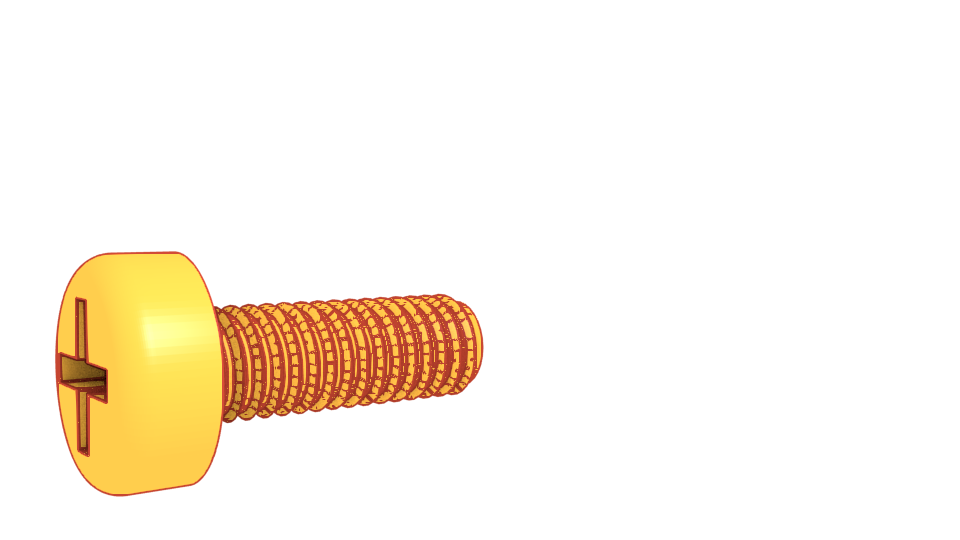
\includegraphics[width=\picwidth]{fig/screws/crosshead-screw-m4x12-orange.png} & Винт M4x12 & 1 шт \\

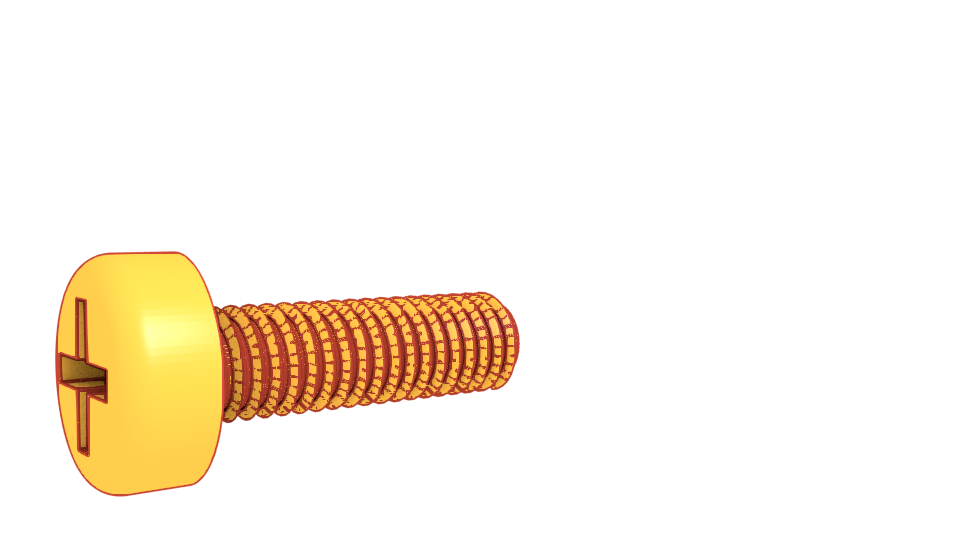
\includegraphics[width=\picwidth]{fig/screws/test/crosshead-screw-m4x14-thr30-cq30-default-iso-orange.png} & Винт M4x14 thr30 cq30 (default ISOThread) & 1 шт \\
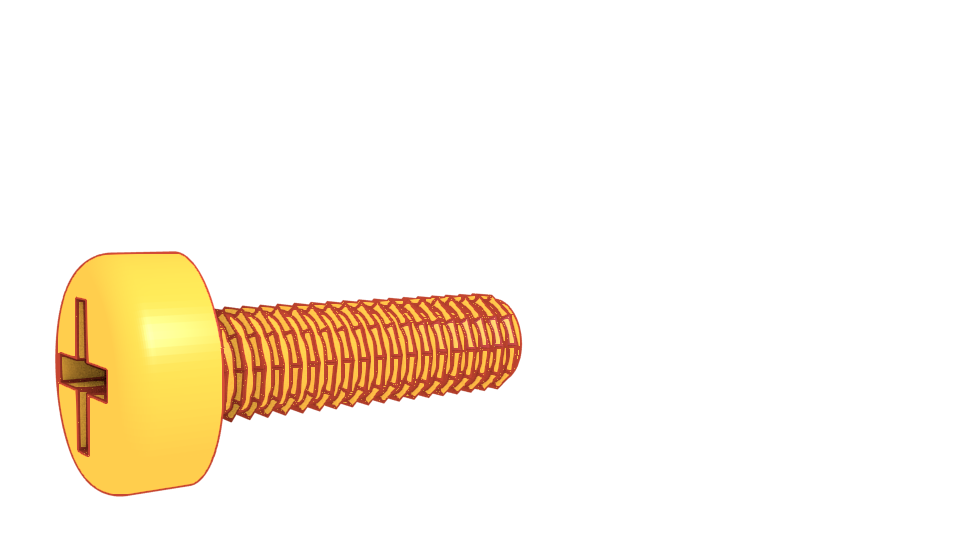
\includegraphics[width=\picwidth]{fig/screws/test/crosshead-screw-m4x14-thr10-cq100-orange.png} & Винт M4x14 thr10 cq100 & 1 шт \\
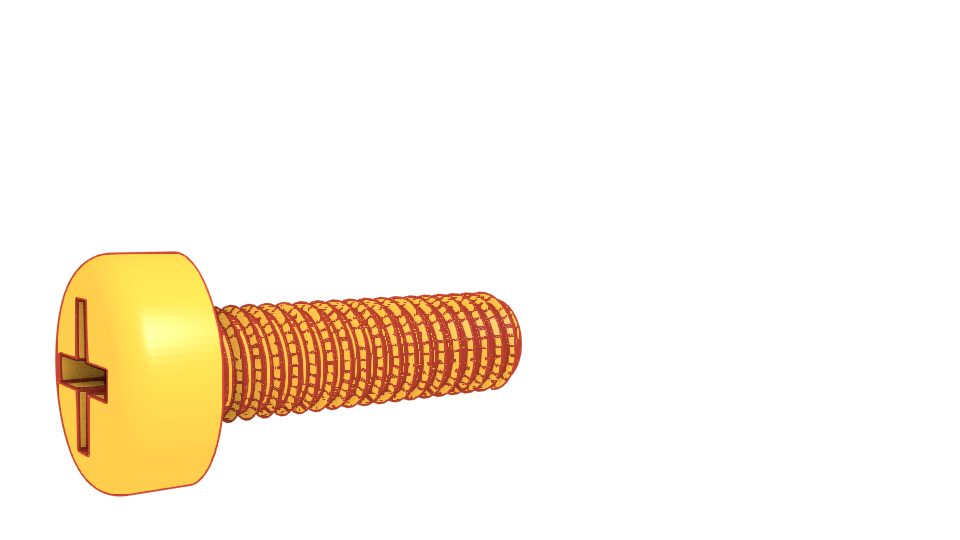
\includegraphics[width=\picwidth]{fig/screws/test/crosshead-screw-m4x14-thr30-cq30-orange.png} & Винт M4x14 thr30 cq30 & 1 шт \\
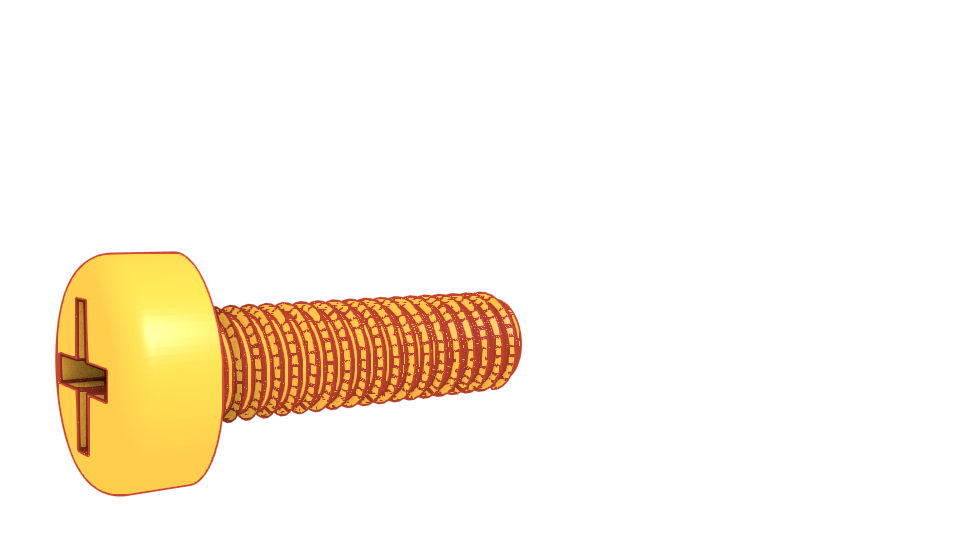
\includegraphics[width=\picwidth]{fig/screws/test/crosshead-screw-m4x14-thr30-cq100-orange.png} & Винт M4x14 thr30 cq100 & 1 шт \\
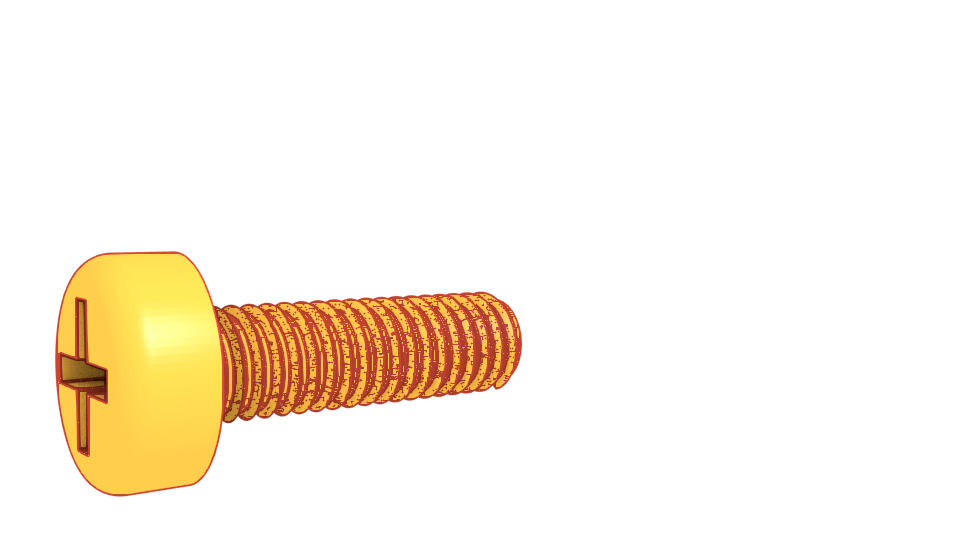
\includegraphics[width=\picwidth]{fig/screws/test/crosshead-screw-m4x14-thr100-cq30-orange.png} & Винт M4x14 thr100 cq30 & 1 шт \\
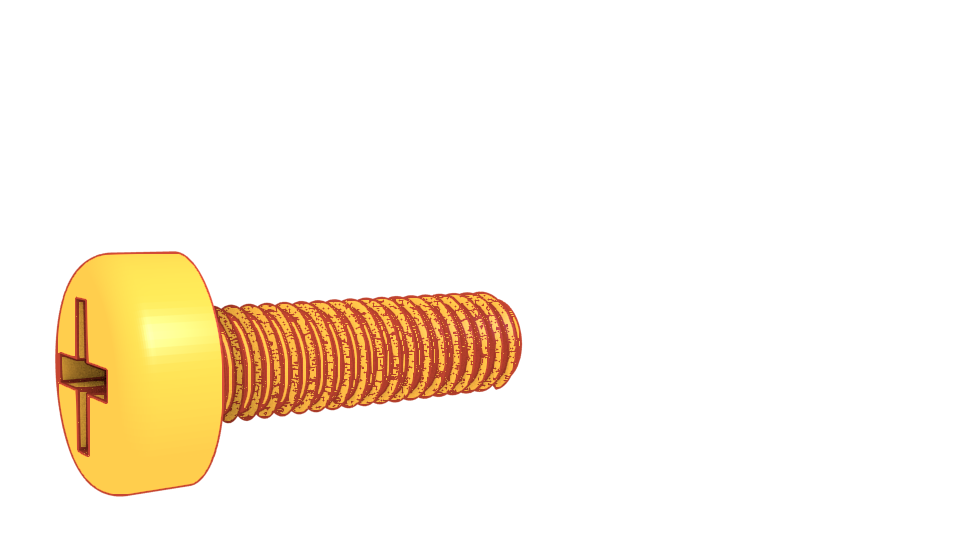
\includegraphics[width=\picwidth]{fig/screws/test/crosshead-screw-m4x14-thr100-cq100-orange.png} & Винт M4x14 thr100 cq100 & 1 шт \\

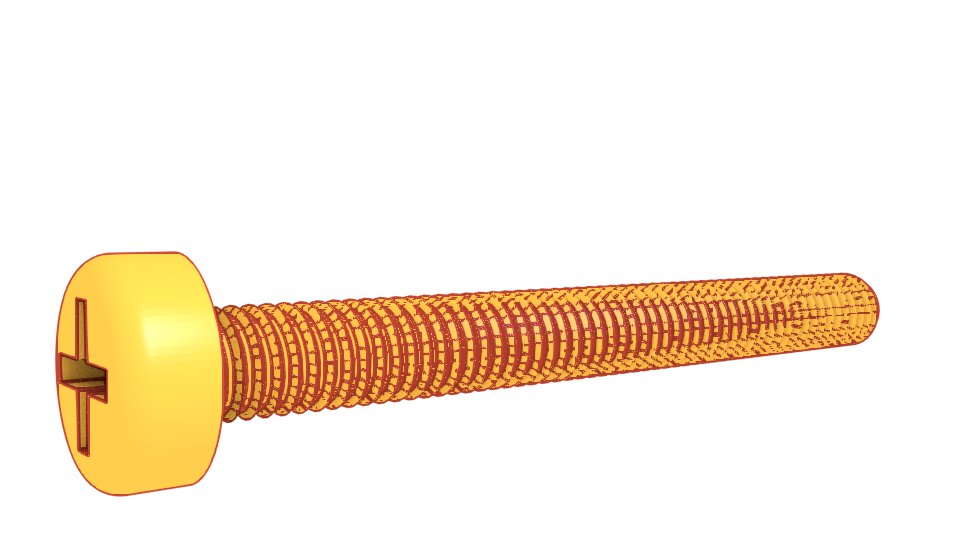
\includegraphics[width=\picwidth]{fig/screws/test/crosshead-screw-m4x40-thr30-cq30-orange.png} & Винт M4x40 thr30 cq30 & 1 шт \\
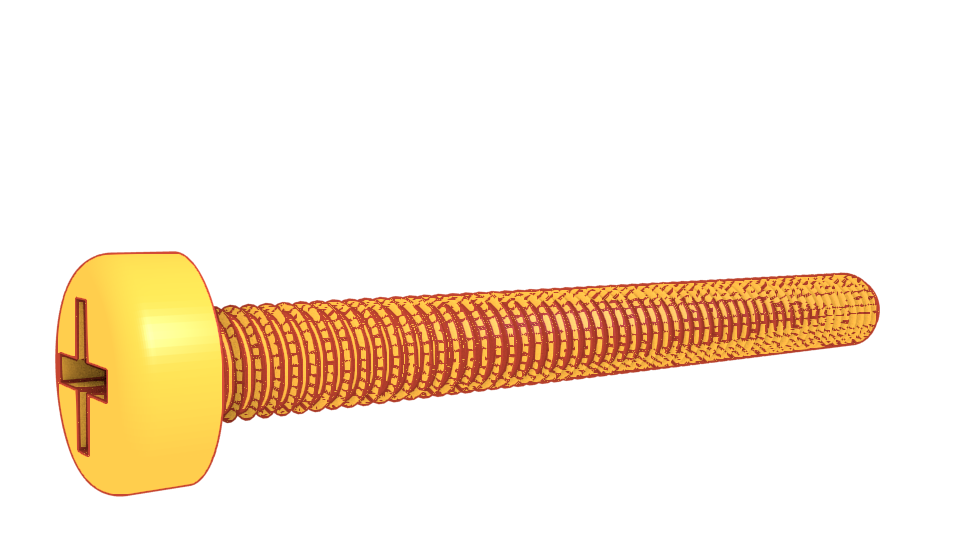
\includegraphics[width=\picwidth]{fig/screws/test/crosshead-screw-m4x40-thr30-cq100-orange.png} & Винт M4x40 thr30 cq100 & 1 шт \\
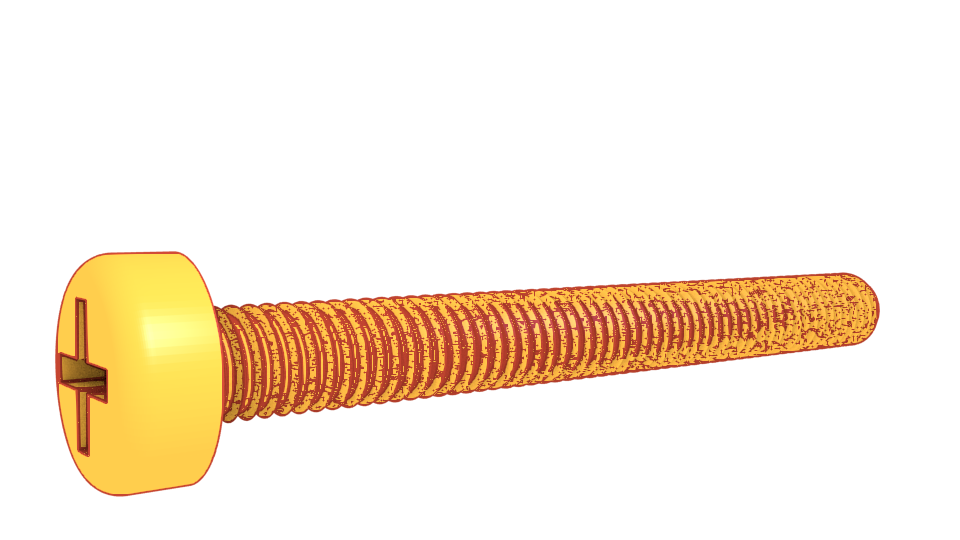
\includegraphics[width=\picwidth]{fig/screws/test/crosshead-screw-m4x40-thr100-cq30-orange.png} & Винт M4x40 thr100 cq30 & 1 шт \\
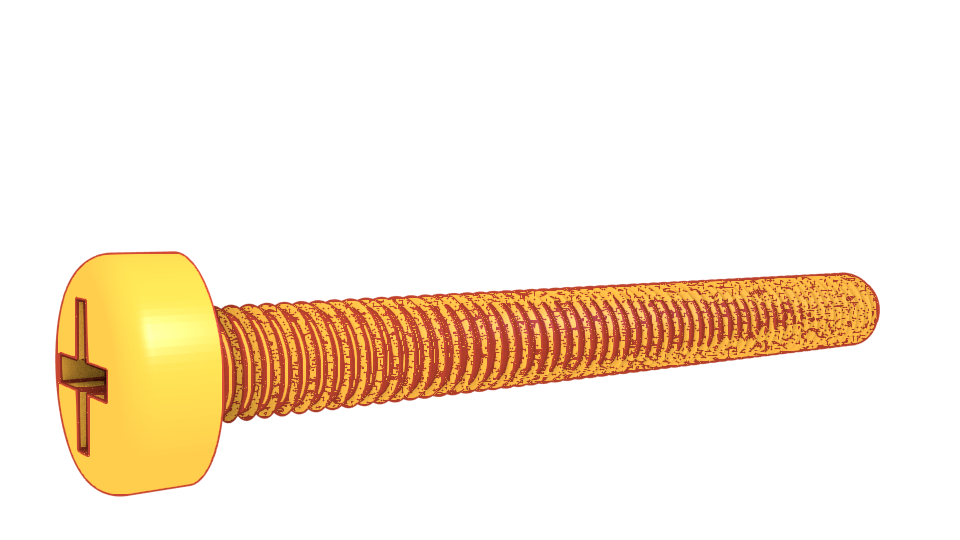
\includegraphics[width=\picwidth]{fig/screws/test/crosshead-screw-m4x40-thr100-cq100-orange.png} & Винт M4x40 thr100 cq100 & 1 шт \\


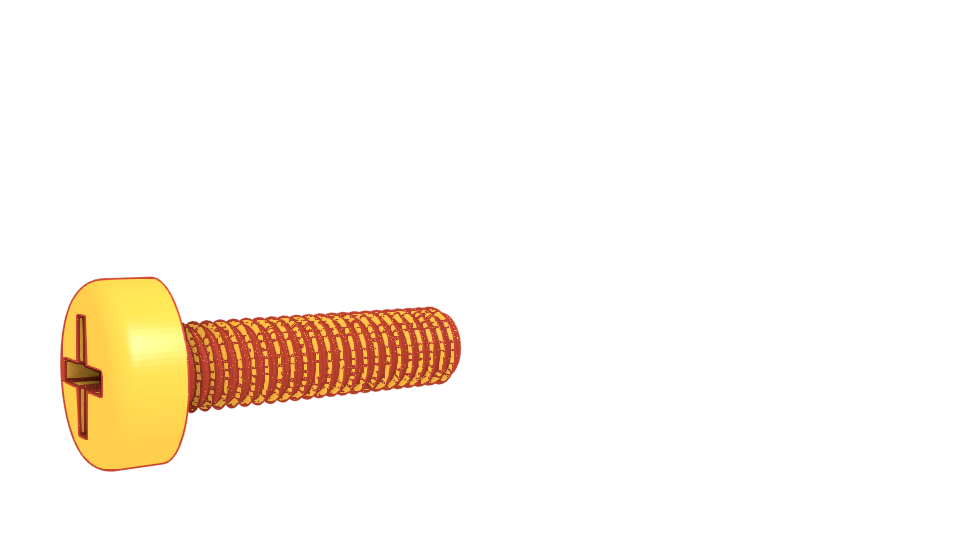
\includegraphics[width=\picwidth]{fig/screws/crosshead-screw-m3x12-orange.png} & Винт M3x12 & 1 шт \\
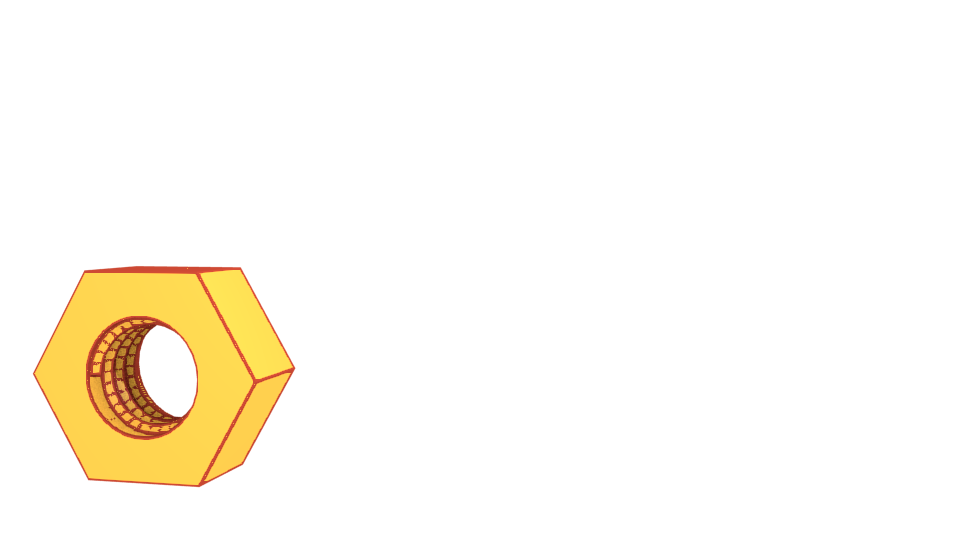
\includegraphics[width=\picwidth]{fig/screws/nut-m4-orange.png} & Гайка M4 & 1 шт \\
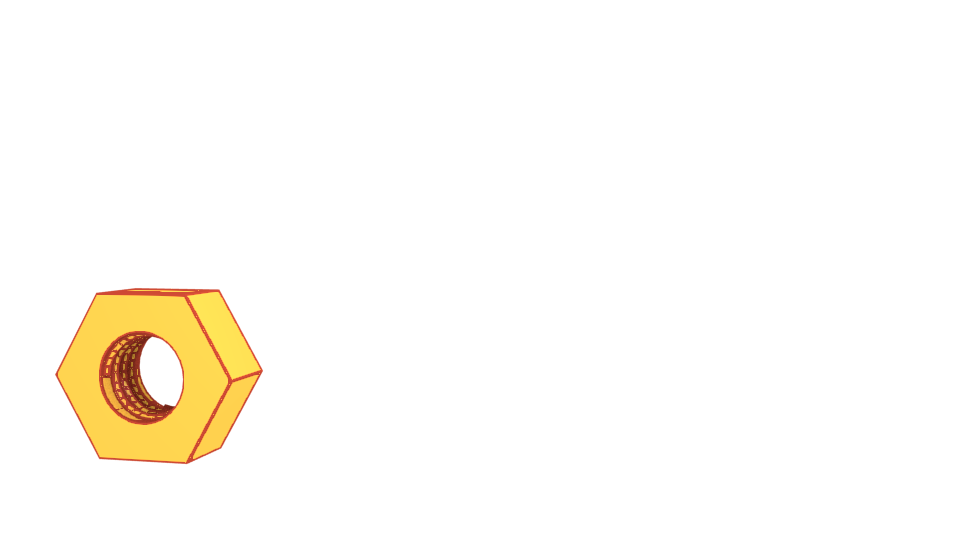
\includegraphics[width=\picwidth]{fig/screws/nut-m3-orange.png} & Гайка M3 & 1 шт \\

  \end{longtabu}   
\end{document}
